\documentclass[a4paper,10pt]{article}
\usepackage[left=2.5cm,right=2.5cm,top=2cm]{geometry}
\usepackage{fontenc}
\usepackage{lmodern}
\usepackage[utf8]{inputenc}
\usepackage[english]{babel}
\usepackage{lmodern}
\usepackage{amsmath}
\usepackage{amsfonts}
\usepackage{amssymb}
\usepackage{amsthm}
\usepackage{graphicx}
\usepackage{color}
\usepackage{xcolor}
\usepackage{url}
\usepackage{textcomp}
\usepackage{listings}
\usepackage{hyperref}

\title{Hardkernel SmartPower3 SCPI manual}
\author{Lukáš Říha}
\date{\today}

\begin{document}
\renewcommand{\labelenumii}{\arabic{enumi}.\arabic{enumii}}
\renewcommand{\labelenumiii}{\arabic{enumi}.\arabic{enumii}.\arabic{enumiii}}
\renewcommand{\labelenumiv}{\arabic{enumi}.\arabic{enumii}.\arabic{enumiii}.\arabic{enumiv}}

\maketitle
\tableofcontents


\section{Introduction}

SmartPower3 is a small power supply designed to provide power supply to up to two connected devices and measure and log the connected devices power consumption. The first firmware versions allowed control of the SmartPower3 via devices buttons, rotary encoder and display. As the system became more mature, some users showed interest in remote control of the power supply. New versions added more refined functionality and SCPI (Standard Commands for Programmable Instruments) capability - effectively enabling (at least partial) remote control of the SmartPower3. This manual tries to describe the commands available in SCPI device mode. 

For more information regarding SCPI and its usage please see the online specification and description available at:\newline\href{http://www.ivifoundation.org/docs/scpi-99.pdf}{http://www.ivifoundation.org/docs/scpi-99.pdf}\newline
and other online resources.

\section{Device modes}

The SmartPower3 device can basically be used in two modes - the default original "buttons and screen" mode and SCPI mode. The default (original) mode tries to be compatible in function with the previous firmware version, while SCPI mode allows programming of the device via serial using SCPI commands and (like the default mode) optionally output logging information to WiFi connected UDP target.

The mode is changed via screen and encoder, on the second device screen, near the bottom. The option is (surprisingly) called \verb|Mode| and allows setting two options:
\begin{enumerate}
    \item Default - provides re-worked two level serial menu that enables setting SmartPower3 functionality.
    \item SCPI - reserves serial connection for SCPI control of the device.
\end{enumerate}

\section{Commands}

\begin{enumerate}
\item IEEE Mandated Commands
    \begin{description}
        \item These commands are required in any SCPI implementation (SCPI std V1999.0 4.1.1).
    \end{description}
    \begin{enumerate}
        \item \hypertarget{cls}{} 
            \begin{verbatim}*CLS\end{verbatim}
            \begin{description}
                Command clears all registers and error queues.
            \end{description}
        \item \begin{verbatim}*ESE\end{verbatim}
		\item \begin{verbatim}*ESE?\end{verbatim}
		\item \begin{verbatim}*ESR?\end{verbatim}
		\item \begin{verbatim}*IDN?\end{verbatim}
		\item \begin{verbatim}*OPC\end{verbatim}
		\item \begin{verbatim}*OPC?\end{verbatim}
        \item \begin{verbatim}*RST\end{verbatim}
            \begin{description}
                Device reset - return device to defined known state. Turns output voltage off and stops logging output.
            \end{description}
        \item \begin{verbatim}*SRE\end{verbatim}
        \item \begin{verbatim}*SRE?\end{verbatim}
        \item \begin{verbatim}*STB?\end{verbatim}
        \item \begin{verbatim}*TST?\end{verbatim}
        \item \begin{verbatim}*WAI"\end{verbatim}
    \end{enumerate}
\item Required SCPI Commands
    \begin{description}
        \item Commands required by Required SCPI commands (SCPI std V1999.0 4.2.1) 
    \end{description}
    \begin{enumerate}
        \item 
            \begin{verbatim}SYSTem:ERRor[:NEXT]?\end{verbatim}
            \begin{description}
                Query removes the last error from error buffer and reports it. Repeatedly calling this query eventually causes the error buffer to become empty.
            \end{description}
        \item 
            \begin{verbatim}SYSTem:ERRor:COUNt?\end{verbatim}
            \begin{description}
                Query reports number of errors since device start-up or last device clear (Please see \hyperlink{cls}{*CLS} command).
            \end{description}
        \item 
            \begin{verbatim}SYSTem:VERSion?\end{verbatim}
            \begin{description}
                Query that reports SCPI standard version this device should adhere to.
            \end{description}
    \end{enumerate}
\item Non-Required SCPI Commands
    \begin{description}
        \item This section contains commands specific to the device and query or control its main functionality.
    \end{description}
    \begin{enumerate}
        \item
            \begin{verbatim}SYSTem:CAPability?\end{verbatim}
            \begin{description}
                Some desc.
            \end{description}
        \item 
            \begin{verbatim}SYSTem:COMMunicate:NETwork:MAC?\end{verbatim}
            \begin{description}
                This query returns the MAC address of the power supply. MAC address consist of two number groups: the first three bytes are known as the Organizationally Unique Identifier (OUI), which is distributed by the IEEE, and the last three bytes are the device’s unique serial number. The six bytes are separated by hyphens. The MAC address is unique to the instrument and cannot be altered by the user.
                \newline
                Return Param <XX-XX-XX-YY-YY-YY>
		    \end{description}
		\item 
		    \begin{verbatim}SYSTem:COMMunicate:NETwork:ADDRess\end{verbatim}
		    \begin{description}
		        This command sets the static address of the power supply.
		    \end{description}
		\item 
		    \begin{verbatim}SYSTem:COMMunicate:NETwork:ADDRess?\end{verbatim}
		    \begin{description}
		        Queries the static IP address of the power supply.
		    \end{description}
		\item 
		    \begin{verbatim}SYSTem:COMMunicate:NETwork:GATE\end{verbatim}
		    \begin{description}
		        This command sets the Gateway IP address of the power supply. Gateway IP address is represented with 4 bytes each having a range of 0-255 separated by dots.
		    \end{description}
		\item 
		    \begin{verbatim}SYSTem:COMMunicate:NETwork:GATE?\end{verbatim}
		    \begin{description}
		        Queries the Gateway IP address of the power supply.
	        \end{description}
	    \item 
	        \begin{verbatim}SYSTem:COMMunicate:NETwork:SUBNet <string>\end{verbatim}
	        \begin{description}
	            This command sets the subnet IP Mask of the power supply.
	        \end{description}
	    \item 
	        \begin{verbatim}SYSTem:COMMunicate:NETwork:SUBNet?\end{verbatim}
	        \begin{description}
		        Queries the value of manually set network subnet mask.
		    \end{description}
		%\item 
		%    \begin{verbatim}[SYSTem][:COMMunicate]:NETwork:PORT\end{verbatim}
		%    \begin{description}
		%        This command sets the Port of the Ethernet module of the power supply.
		%    \end{description}
		%\item
		%    \begin{verbatim}[SYSTem][:COMMunicate]:NETwork:PORT?\end{verbatim}
		%    \begin{description}
		%        *
		%    \end{description}
		%\item 
		%    \begin{verbatim}// [SYSTem][:COMMunicate]:NETwork:HOSTname?\end{verbatim}
		%    \begin{description}
		%        This query reads the host name of the Ethernet communications module.
		%    \end{description}
		\item 
		    \begin{verbatim}SYSTem:COMMunicate:NETwork:DHCP\end{verbatim}
		    \begin{description}
		        This command sets the DHCP operating mode of the Ethernet module. If DHCP is set to 1, the module will allow its IP address to be automatically set by the DHCP server on the network. If DHCP is set to 0, the default IP address is set according to .
		    \end{description}
		\item 
		    \begin{verbatim}SYSTem:COMMunicate:NETwork:DHCP?\end{verbatim}
		    \begin{description}
		        This query reports the DHCP operating mode currently set.
		    \end{description}
		\item 
		    \begin{verbatim}SYSTem:COMMunicate:SOCKet:ADDRess\end{verbatim}
		    \begin{description}
		        Command sets logging target IP address (UDP logging server address). 
		    \end{description}
		\item 
		    \begin{verbatim}SYSTem:COMMunicate:SOCKet:ADDRess?\end{verbatim}
		    \begin{description}
		        Queries logging target IP address (UDP logging server address).
		    \end{description}
		\item
		    \begin{verbatim}SYSTem:COMMunicate:SOCKet:PORT\end{verbatim}
		    \begin{description}
		        Command sets logging target port (UDP logging server port).
		    \end{description}
		\item 
		    \begin{verbatim}SYSTem:COMMunicate:SOCKet:PORT?\end{verbatim}
		    \begin{description}
		        Queries logging target port (UDP logging server port).
		    \end{description}

		\item
		    \begin{verbatim}SYSTem:COMMunicate:SOCKet:CONNect\end{verbatim}
		    \begin{description}
		        Command connects to the target socket. In case of SmartPower3 and UDP WiFi logging, this basically means connecting to WiFi network, the same way one can connect by moving cursor over WiFi icon when disconnected and pressing encoder button.
		    \end{description}
		\item 
		    \begin{verbatim}SYSTem:COMMunicate:SOCKet:DISConnect\end{verbatim}
		    \begin{description}
		        Command disconnects to the target socket. In case of SmartPower3 and UDP WiFi logging, this basically means disconnecting from WiFi network, the same way one can disconnect by moving cursor over WiFi icon when connected and pressing encoder button.
		    \end{description}

        \item
            \begin{verbatim}SYSTem:COMMunicate:SOCKet:FEED <data_handle>\end{verbatim}
            \begin{description}
                Connect or disconnect the logging output to connected socket - WiFi.
                The data handle parameter can be one of two values:
                    \item \verb|LOG| - connect the logging output
                    \item \verb|NONE| - disconnect the logging output
            \end{description}
        \item
            \begin{verbatim}SYSTem:COMMunicate:SOCKet:FEED?\end{verbatim}
            \begin{description}
                Report what data source is connected to the logging output.
                The result can be one of the following values:
                    \item \verb|LOG|
                    \item \verb|NONE|
            \end{description}
        \item
            \begin{verbatim}SYSTem:COMMunicate:SERial:FEED <data_handle>\end{verbatim}
            \begin{description}
                Connect the logging output to connected serial port.
                The data handle parameter can be one of two values:
                    \item \verb|LOG| - connect the logging output
                    \item \verb|NONE| - disconnect the logging output
            \end{description}
        \item
            \begin{verbatim}SYSTem:COMMunicate:SERial:FEED?\end{verbatim}
            \begin{description}
                Report what data source is connected to the logging output.
                The result can be one of the following values:
                    \item \verb|LOG|
                    \item \verb|NONE|
            \end{description}
        \item 
            \begin{verbatim}SYSTem:COMMunicate:RLSTate\end{verbatim}
            \begin{description}
                Sets the device operation mode. Equivalent to the \verb|Mode| screen menu item.
                Acceptable options are:
                \item \verb|LOCal|
                    - Corresponds to the \verb|Default| menu selection.
                \item \verb|REMote|
                    - Corresponds to the \verb|SCPI| menu selection.
            \end{description}
        \item 
            \begin{verbatim}SYSTem:COMMunicate:RLSTate?\end{verbatim}
            \begin{description}
                Queries the selected device operation mode. Equivalent to the \verb|Mode| screen menu item.
                Possible responses are:
                \item \verb|LOCal|
                    - Corresponds to the \verb|Default| menu selection.
                \item \verb|REMote|
                    - Corresponds to the \verb|SCPI| menu selection.
            \end{description}
            
            
            
		% STATus:OPERation:CONDition?
		% STATus:OPERation:ENABle
		% STATus:OPERation:ENABle?

		%\item 
		%    \begin{verbatim}STATus:QUEStionable[:EVENt]?\end{verbatim}
		%    \begin{description}
		%        TBD
		%    \end{description}
		%\item
		%    \begin{verbatim}// STATus:QUEStionable:CONDition?\end{verbatim}
		%    \begin{description}
		%        TBD
		%    \end{description}
		%\item 
		%    \begin{verbatim}STATus:QUEStionable:ENABle\end{verbatim}
		%    \begin{description}
		%        TBD
		%    \end{description}
		%\item 
		%    \begin{verbatim}STATus:QUEStionable:ENABle?\end{verbatim}
		%    \begin{description}
		%        TBD
		%    \end{description}

		%\item 
		%    \begin{verbatim}STATus:PRESet\end{verbatim}
		%    \begin{description}
		%        TBD
		%    \end{description}

		%/* DMM */
		\item \hypertarget{FETCh}{}
		    \begin{verbatim}FETCh[:SCALar]:VOLTage[:DC]? [expected_value, [resolution,]] <channel_list>\end{verbatim}
		    \begin{description}
		        Command allows reading voltage on channel specified by \verb|<channel_list>|. Parameter \verb|expected_value| has no use in this case and is included for reasons of compatibility. Parameter \verb|resolution| allows specifying the resolution of the result. If ommited, the result is returned in Volts. Parameter \verb|<channel_list>| allows specifying which channel(s) result should be read. The order of the channels is important - results are returned in that order.
		        \newline If all parameters are ommited, the command will return value for channel 1, in Volts.
		        \item Example 1:
		            \begin{verbatim}FETCh:VOLTage? 1 V, 0.001V, (@1:3)\end{verbatim} will return voltage read on all three channels (including the power supply supply channel), in milliVolts, in order of channel 1, 2, 3.
		        \item Example 2:
		            \begin{verbatim}FETCh:VOLTage? (@3,1)\end{verbatim} will return voltage read on channels 3 and 1 (in that order), in units of Volts.
		    \end{description}
		\item 
		    \begin{verbatim}FETCh[:SCALar]:CURRent[:DC]? [expected_value, [resolution,]] <channel_list>\end{verbatim}
		    \begin{description}
		        Command allows reading of current on channel specified by \verb|<channel_list>|, averaged over 2 samples. If \verb|resolution| is not specified, the value is returned in Amperes.
		        Parameter \verb|<channel_list>| allows specifying which channel(s) result should be read. The order of the channels is important - results are returned in that order.
		        \newline If all parameters are ommited, the command will return value for channel 1, in Amperes.
		        \item Example 1:
		            \begin{verbatim}FETCh:CURRent? 1 A, 0.001A, (@1:3)\end{verbatim} will return current read on all three channels (including the power supply supply channel), in milliAmperes, in order of channel 1, 2, 3.
		        \item Example 2:
		            \begin{verbatim}FETCh:CURRent? (@3,1)\end{verbatim} will return current read on channels 3 and 1 (in that order), in units of Amperes.
		    \end{description}
		\item 
		    \begin{verbatim}FETCh[:SCALar]:POWer[:DC]? [expected_value, [resolution,]] <channel_list>\end{verbatim}
		    \begin{description}
		        Command allows reading power on channel specified by \verb|<channel_list>|. Parameter \verb|expected_value| has no use in this case and is included for reasons of compatibility. Parameter \verb|resolution| allows specifying the resolution of the result. If ommited, the result is returned in Watts. Parameter \verb|<channel_list>| allows specifying which channel(s) result should be read. The order of the channels is important - results are returned in that order.
		        \newline If all parameters are ommited, the command will return value for channel 1, in Watts.
		        \item Example 1:
		            \begin{verbatim}FETCh:POWer? 1 V, 0.001V, (@1:3)\end{verbatim} will return power read on all three channels (including the power supply supply channel), in milliWatts, in order of channel 1, 2, 3.
		        \item Example 2:
		            \begin{verbatim}FETCh:POWer? (@3,1)\end{verbatim} will return power read on channels 3 and 1 (in that order), in units of Watts.
		    \end{description}

		\item
		    \begin{verbatim}[SOURce#]:CURRent <numeric_value>\end{verbatim}
		    \begin{description}
		        Sets output current on source \verb|#|. If \verb|#| is ommited, the default value is 1.
		        \newline
		        \verb|<numeric_value>| is the value that should be set on the device. Default unit is Amperes. Other possible values include \verb!MIN|MAX!, which set minimum and maximum persmissible value, respectively. Another option, if you decide to use \verb|A| unit is to specify units as fractions, such as \verb|mA| (milliAmperes) or \verb|UA| (microAmperes). 
		    \end{description}
		\item 
		    \begin{verbatim}[SOURce#]:CURRent?\end{verbatim}
		    \begin{description}
		        Querries the output current set on channel \verb|#|. Note that this differs from the \hyperlink{FETCh}{FETCh} series of commands in that no measurements are taken and value set by \verb|[SOURce#]:CURRent| is returned.
		        \newline
		        Returns value in Amperes.
		    \end{description}
		\item 
		    \begin{verbatim}[SOURce#]:VOLTage <numeric_value>\end{verbatim}
		    \begin{description}
		        Sets output voltage on source \verb|#|. If \verb|#| is ommited, the default value is 1.
		        \newline
		        \verb|<numeric_value>| is the value that should be set on the device. Default unit is Volts. Other possible values include \verb!MIN|MAX!, which set minimum and maximum persmissible value, respectively. Another option, if you decide to use \verb|V| unit is to specify units as fractions, such as \verb|mV| (milliVolts) or \verb|UV| (microVolts). 
		    \end{description}
		\item 
		    \begin{verbatim}[SOURce#]:VOLTage?\end{verbatim}
		    \begin{description}
		        Querries the output voltage set on channel \verb|#|. Note that this differs from the \hyperlink{FETCh}{FETCh} series of commands in that no measurements are taken and value set by \verb|[SOURce#]:VOLTage| is returned.
		        \newline
		        Returns value in Amperes.
		    \end{description}

		\item 
		    \begin{verbatim}OUTPut#[:STATe] <parameter>\end{verbatim}
		    \begin{description}
		        This command turns the output channel \verb!#! on or off. If \verb|#| is ommited, the command defaults to channel number 1.
		        \newline Possible parameter value is one of \verb!ON|1|OFF|0!.
		    \end{description}
		\item 
		    \begin{verbatim}OUTPut#[:STATe]?\end{verbatim}
		    \begin{description}
		        This query returns the output states of channel \verb!#!. Returns 0 or 1.
		    \end{description}
    \end{enumerate}
\end{enumerate}

\section{Python Examples}

The power supply in SCPI mode can also be controlled by various VISA implementations. This enables the user to programmatically perform and repeat various test and measurements, that might otherwise be quite complicated or outright impossible with sufficient precision.

The following is a simple example of how the device might be used.

More information on how to use PyVISA can be found at\newline
\href{https://pyvisa.readthedocs.io/en/latest/introduction/index.html}{https://pyvisa.readthedocs.io/en/latest/introduction/index.html}.

\subsection{Prerequisites}

It is expected that you have Python3, PyVISA and backed installed. We are going to use PyVISA-py for the backend.

The exact steps how to install these prerequisites depend on your selection of operating system and its version. For example, most Linux distributions will have Python installed by default, so its installation might be skipped.

Once Python is installed, you could, for example, install the remaining dependencies for the current user by running the following in terminal:
\begin{verbatim}
    pip install -U pyvisa pyvisa-py
\end{verbatim}

\subsection{Connecting to the Power Supply}

The next step is to connect to the SmartPower3 power supply. To do so, please follow these steps:
\begin{enumerate}

    \item Connect SmartPower3 to your computer using serial cable.
    \item On the setting screen, set SmartPower3 to \verb|SCPI| mode.
    \item Open your terminal application and start Python interpreter by typing:\newline\verb|python|
    \item Import PyVISA and connect by typing the following
    \begin{verbatim}
        >>> import pyvisa
        >>> rm = pyvisa.ResourceManager()
        >>> rm.list_resources()
        ('ASRL/dev/ttyUSB0::INSTR')
        >>> inst = rm.open_resource('ASRL/dev/ttyUSB0::INSTR')
        >>> print(inst.query('*IDN?'))
    \end{verbatim}
    The \verb|('ASRL/dev/ttyUSB0::INSTR')| string will most likely be different in your case. You might even have more devices listed, depending on your hardware. That is OK, just select the one that corresponds to your serial connection.
    
    The last command (\verb|print(inst.query("*IDN?"))|) should result in the terminal printing out the power supply identification, which should look similar to 
    
    \verb|Hardkernel Co Ltd,SmartPower3,<mac_address>,Build date: Jul 19 2023 19:32:24|, where \verb|<mac_address>| will be the WiFi module MAC address (a string similar to \newline\verb|94:3C:C6:CC:AA:78|) and the Build date will reflect your current firmware version.
    \item In case the last command didn't produce the desired result and you got timeout error response, there are couple things you can check to remedy the situation:
    \begin{enumerate}
        \item Check that the device is in SCPI mode.
        \item Check device serial baud rate. It is quite possible that your SmartPower3 is set to a higher baud rate than 9600, which is PyVISA default. To set correct baud rate, you can use the following command:
        \begin{verbatim}
            inst.baud_rate = 115200
        \end{verbatim}
        where \verb|115200| should be changed to the actual value set on your SmartPower3.
        \item It is possible that the response was followed by an empty line. In such a case, there is a mismatch between line endings returned by the device and line endings that PyVISA expects. That can be remedied by issuing the following command:
        \begin{verbatim}
            inst.read_termination = '\r\n'
        \end{verbatim}
    \end{enumerate}
    For more troubleshooting info please see PyVISA documentation available\newline at \href{https://pyvisa.readthedocs.io/en/latest/introduction/communication.html\#}{https://pyvisa.readthedocs.io/en/latest/introduction/communication.html\#}.
      
\end{enumerate}
\subsection{Doing Something Usefull}
Once you have succeded in issuing the identification command and getting a proper response, we can get to something more useful.
\subsubsection{Doing a Voltage Sweep}
Let's suppose that you have just finished a construction of a new hardware device that is supposed to be powered by 12 Volts DC. But you also want to check how the device behaves at a lower voltage, gradually bringing the voltage up from 5V to the full 12V. That could be achieved by the following commands:
\begin{verbatim}
    # by now, you have pyvisa imported and are connected to the device
    import time
    start_voltage = 5
    end_voltage = 12
    inst.write(f'source1:volt {start_voltage}')  # the starting voltage on channel 1
    # uncommenting the next line turns channel 1 on and the sweep is done under power
    # it is advisable to first check the functionality of your program
    # with the output turned off, in case there is a mistake
    # inst.write('output1 on')
    while(start_voltage <= end_voltage):
        print(f'start_voltage = {start_voltage}')
        inst.write(f'source1:volt {start_voltage}')
        start_voltage += 1  # increase the value of start_voltage by 1
        time.sleep(2)  # wait 2 seconds
\end{verbatim}

The example above is rather rudimentary and does not use the possibilities of the device to its full extent.

If you wanted to set values on a finer scale than whole Volts and not use Python float data type - which is advisable, as it can lead to unpredictable results - you could modify the above script as follows:

\begin{verbatim}
    # by now, you have pyvisa imported and are connected to the device
    import time
    start_voltage = 3000  # the value represented in milliVolts 
    end_voltage = 5000  # the value represented in milliVolts
    inst.write(f'source1:volt {start_voltage}mV')  # note the added unit of mV
    # uncommenting the next line turns channel 1 on and the sweep is done under power
    # it is advisable to first check the functionality of your program
    # with the output turned off, in case there is a mistake
    # inst.write('output1 on')
    while(start_voltage <= end_voltage):
        print(f'start_voltage in Volts = {start_voltage/1000}')
        inst.write(f'source1:volt {start_voltage}mV')  # note the added unit of mV
        # increase the value of start_voltage by 20mV, which is the smallest
        # possible step in this voltage range
        start_voltage += 20
        time.sleep(2)  # wait 2 seconds
\end{verbatim}

\subsubsection{Plotting Power Data From Measurements on Channel 1}
    The \verb|contrib/SCPI_examples| directory of Smartpower3 git repository contains file\newline
    \verb|sp3-scpi-datalogger.py| which does exactly what the subtitle advertises.
    
    But before you use it, you should be aware of a couple of important points:
    \begin{enumerate}
        \item 
            Check what voltage your device operates on. The file sets output voltage to 5.1V (required for Raspberry Pi 4), so if your device operates on other voltage, change \verb|device_input_voltage| variable in the \verb|run| function to the required value.
        \item 
            The script expects the device to be connected to the first (left) channel.
        \item 
            The script expects that you use Serial connection to your SmartPower3 and it lets you choose your serial device.
        \item
            It asks you how long you want to run the logging - plese enter numeric value, seconds.
        \item
            Before you run the script with your device connected to SmartPower3, please run the script without the device to make sure everything is working as expected, the power is set to correct level etc. Doublecheck everything.
        \item 
            The script saves logged data to intermediate .csv file in the same directory as the script. You might want to use that file for further analysis.
        \item 
            The scrip is pretty basic and definitely can be improved upon - don't hesitate to modify it to suit your needs. But please doublecheck before powering your device.
    \end{enumerate}
    If everything goes well, the script will output window with power plot similar to Figure 1.
    \begin{figure}
        \begin{center}
            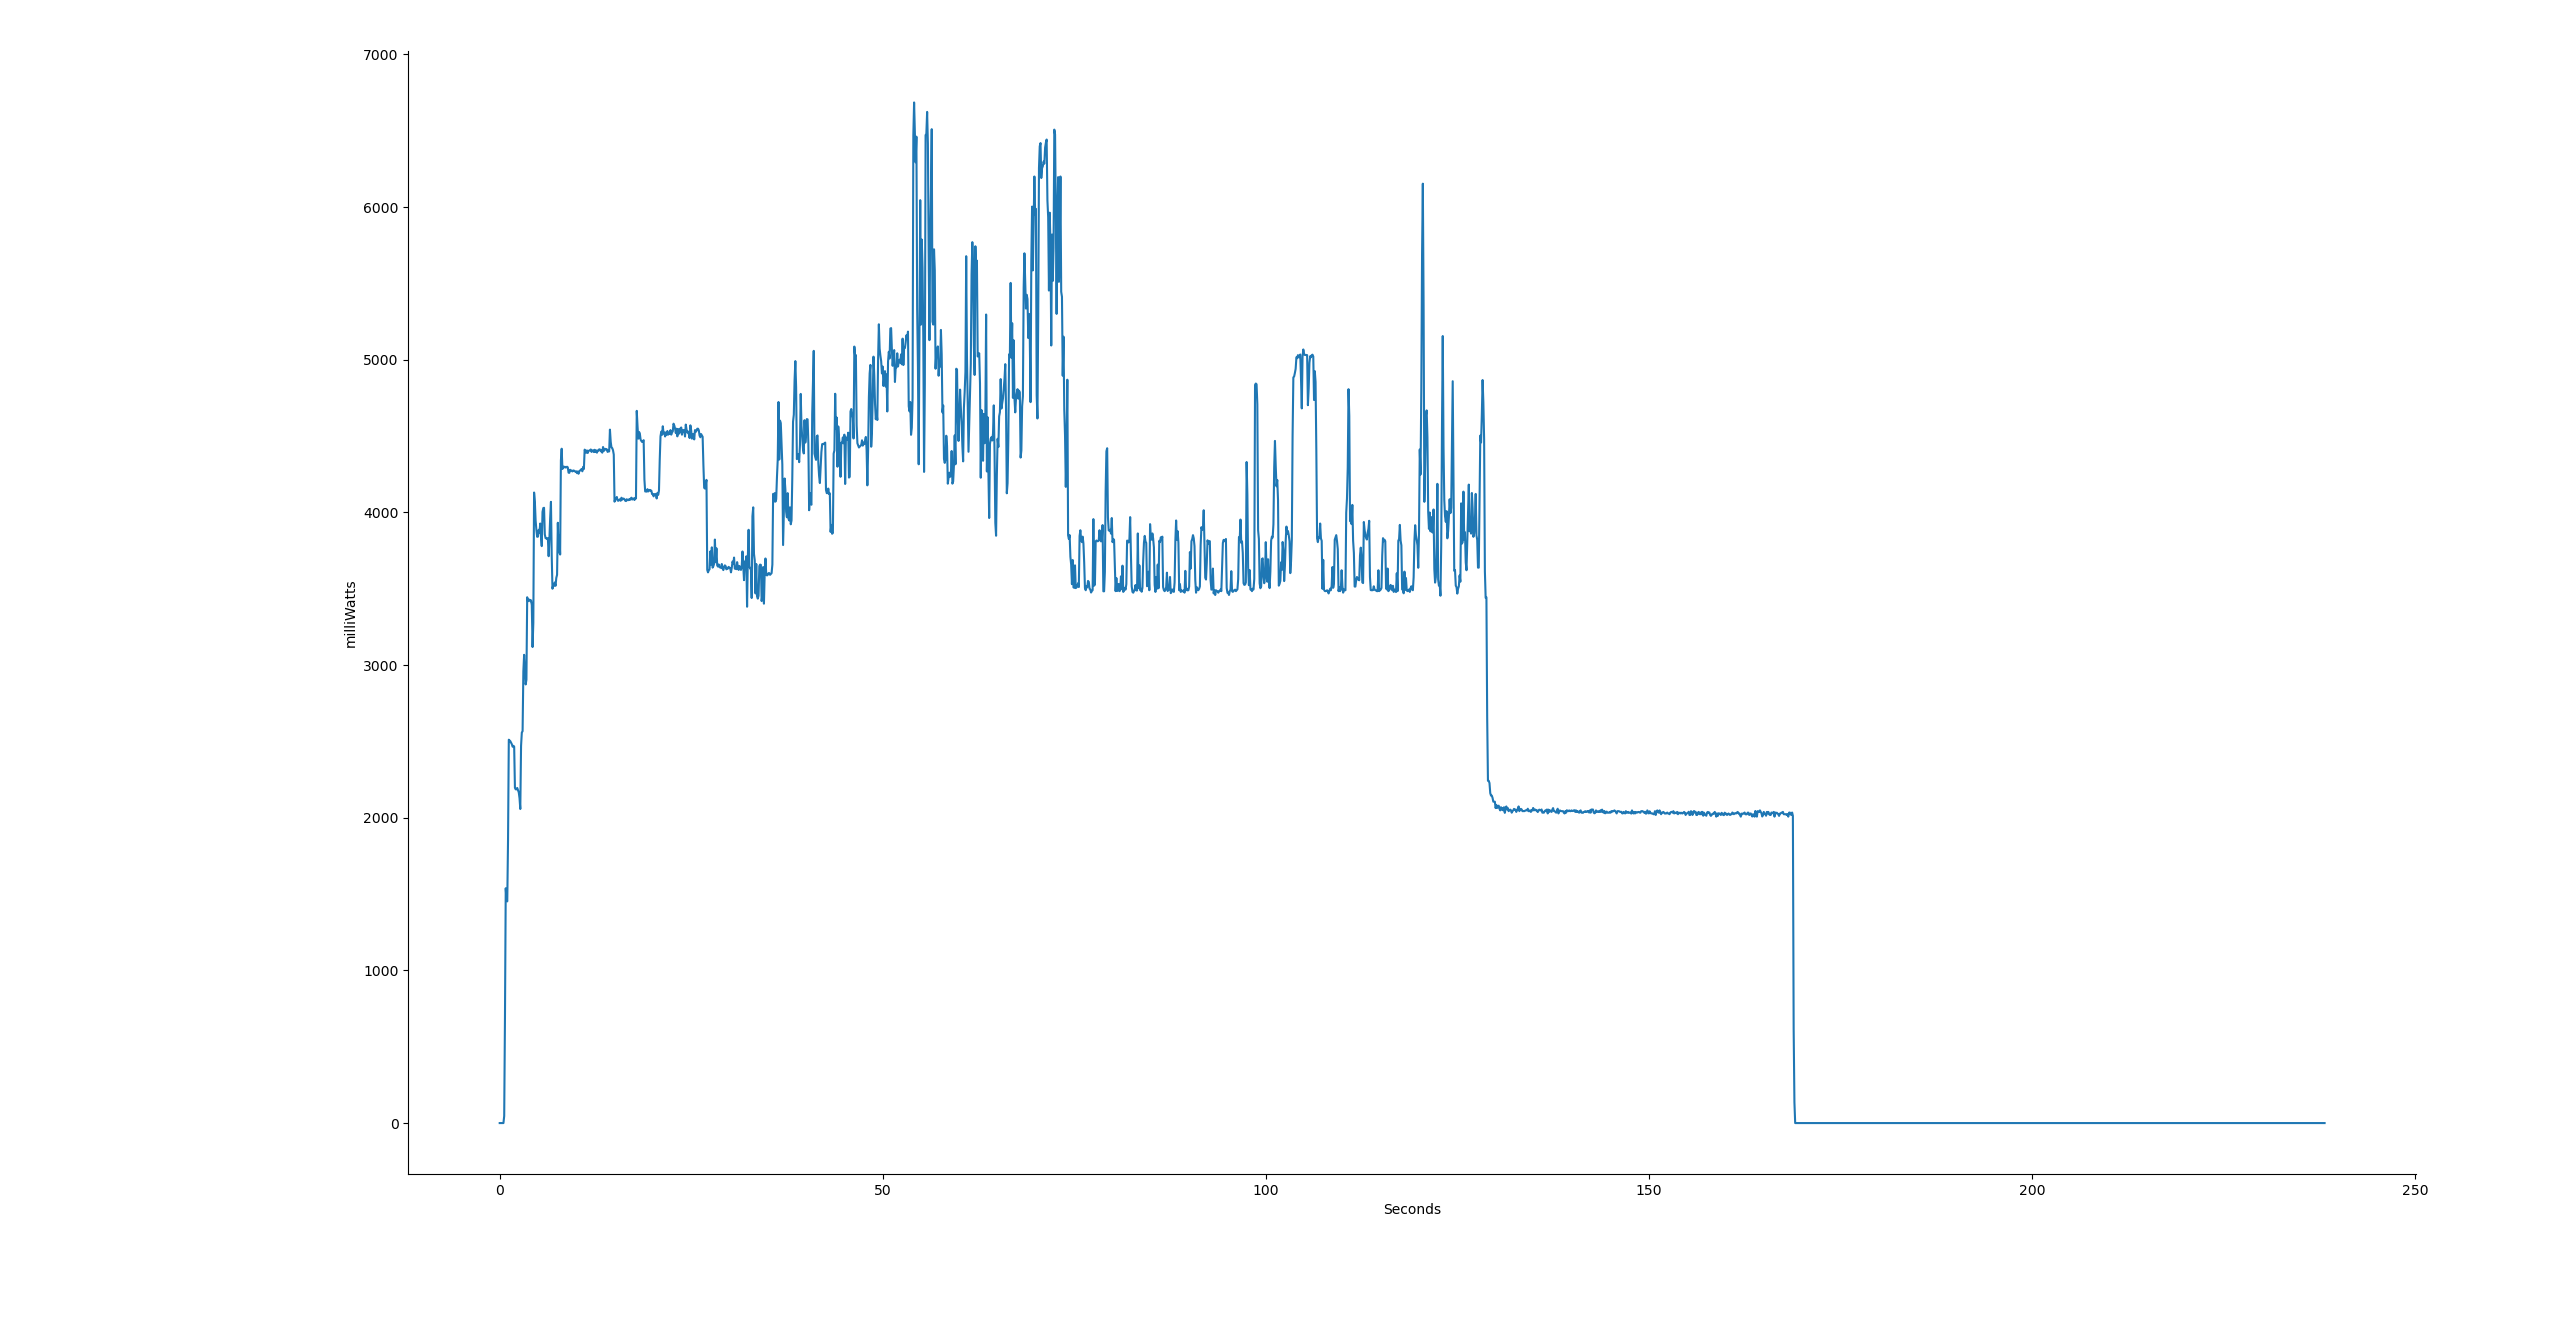
\includegraphics[scale=0.24]{Figure_1.png}
            \caption{Script output}
        \end{center}
    \end{figure}
    
    If things don't go as planned, please check the following:
    \begin{enumerate}
    \item 
        Check that the device mode is set to SCPI. If not and you try to use PyVisa, you will most likely get complains about read method not having read termination and \verb|>>> Unknown Command <<<|.
    \item 
        Check the device you try to power is connected to the correct channel.
    \end{enumerate}

\end{document}